\chapter{Gambar dan Laporan Kinerja Tambahan}
\label{appendix:additional_results}

Bagian ini menyajikan visualisasi tambahan mengenai arsitektur sirkuit kuantum, analisis pengaruh kedalaman sirkuit, serta laporan ringkasan kinerja portofolio.

\section{Arsitektur Sirkuit Kuantum}
\label{appendix:circuit_diagram}
Gambar \ref{fig:circuit_diagram} mengilustrasikan sirkuit kuantum yang digunakan dalam optimasi portofolio dengan \textit{Hardware-Efficient Ansatz}.

\begin{figure}[H]
    \centering
    
\includegraphics[width=0.8\textwidth]{GTQuantumInvest/Hasil_N2_GT/rangkaian_kuantum_depth2_N2.png}
    \caption{Rangkaian Sirkuit Kuantum dengan Kedalaman (\textit{Depth}) 2}
    \label{fig:circuit_diagram}
\end{figure}

\section{Analisis Kedalaman Sirkuit (\textit{Depth Analysis})}
\label{appendix:depth_analysis}
Grafik pada Gambar \ref{fig:depth_energy_plot} menunjukkan hubungan antara peningkatan kedalaman sirkuit terhadap pencapaian energi Hamiltonian minimum.

\begin{figure}[H]
    \centering
    
\includegraphics[width=0.8\textwidth]{GTQuantumInvest/Hasil_N2_GT/grafik_depth_per_window_N2.png}
    \caption{Grafik Performa Energi Hamiltonian terhadap Variasi \textit{Depth}}
    \label{fig:depth_energy_plot}
\end{figure}

\section{Ringkasan Kinerja Strategi (\textit{Backtest Report})}
\label{appendix:backtest_report}
Berikut adalah ringkasan performa kumulatif dan metrik risiko dari strategi GT-VQE dibandingkan dengan tolok ukur pasar.

\begin{figure}[H]
    \centering
    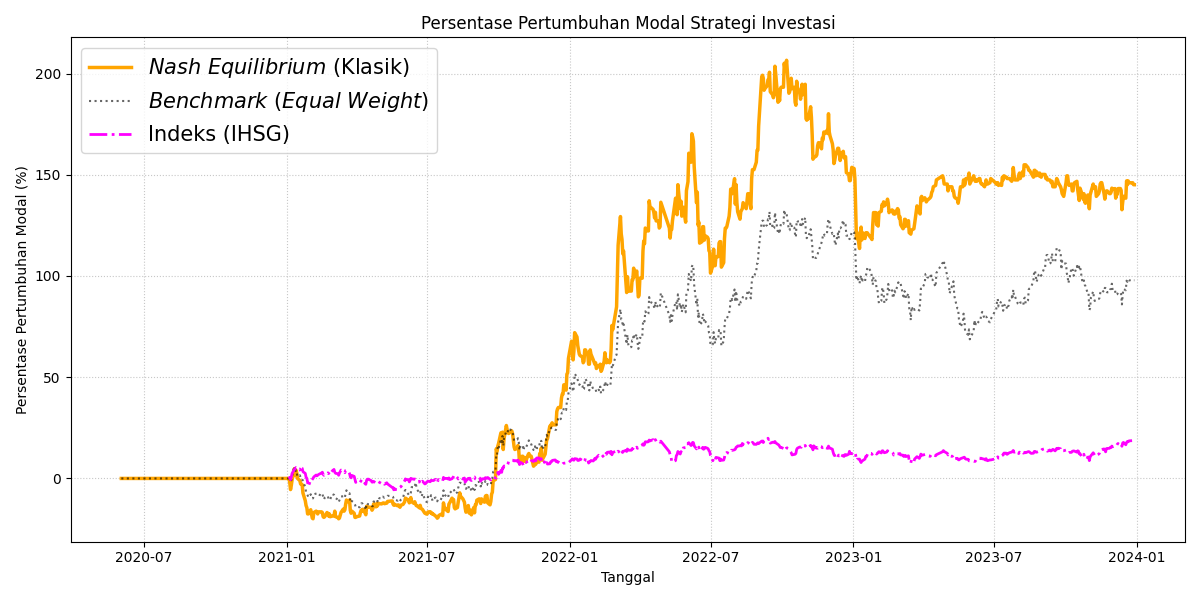
\includegraphics[width=0.85\textwidth]{GTQuantumInvest/Hasil_N2_GT/hasil_backtest_nash_N2.png}
    \caption{Kurva Performa Kumulatif (\textit{Backtesting}) Strategi \textit{Nash Equilibrium} (Klasik)}
    \label{fig:backtest_curve_nash}
\end{figure}

\begin{figure}[H]
    \centering
    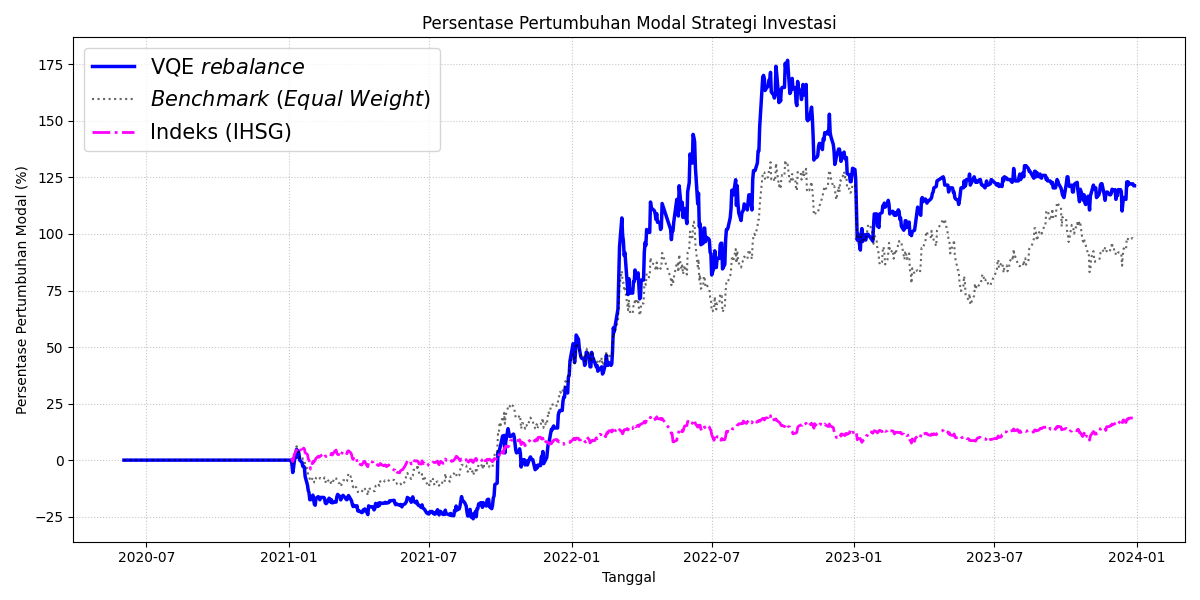
\includegraphics[width=0.85\textwidth]{GTQuantumInvest/Hasil_N2_NoGT/hasil_backtest_vqe_N2.png}
    \caption{Kurva Performa Kumulatif (\textit{Backtesting}) Strategi \textit{Quantum VQE} (Tanpa \textit{Warm-Start})}
    \label{fig:backtest_curve_vqe_nogt}
\end{figure}

\begin{figure}[H]
    \centering
    
\includegraphics[width=0.85\textwidth]{GTQuantumInvest/Hasil_N2_GT/hasil_backtest_vqe_N2.png}
    \caption{Kurva Performa Kumulatif (\textit{Backtesting}) Strategi \textit{Quantum VQE} (Dengan \textit{Warm-Start} GT)}
    \label{fig:backtest_curve_vqe_gt}
\end{figure}
